\documentclass{report}
\usepackage{ccicons}
\usepackage{hyperref}
\usepackage{graphicx}
\usepackage[utf8]{inputenc}
\usepackage{todonotes}
\usepackage{textcomp}
\usepackage{amsmath}
\usepackage{tcolorbox}
\usepackage{wrapfig}

\title{TheBounty Renderer: Official documentation}
\author{TheBounty Renderer Team \and YafaRay Team}

\newcommand{\note}[1]{\begin{tcolorbox}[title=Note] #1\end{tcolorbox}}
\newcommand{\tbrref}[1]{Section~\ref{#1} on page~\pageref{#1}}
\newcommand{\tbrchapref}[1]{Chapter~\ref{#1} on page~\pageref{#1}}

\begin{document}
\begin{titlepage}
    \centering
    \vfill
    {
        
\includegraphics[width=.9\textwidth]{images/logo.png} % also works with logo.pdf
        {\Huge Official documentation}\\
        \Large
        \vskip2cm
        the TheBounty Renderer Team\\
        {\large and}
        \\
        the Yafaray Team\\
    }    
    \vfill
    \vfill
    The Thebounty Renderers User's Guide by \url{www.thebountyrenderer.org} and \url{www.yafaray.org} is licensed under a Creative Commons Attribution-Share Alike 4.0 International License. For further information please refer to \url{http://creativecommons.org/licenses/by-sa/4.0/}.
    \begin{flushright}
    \ccbysa
    \end{flushright}
\end{titlepage}
\tableofcontents
\chapter*{Introduction}
 \addcontentsline{toc}{chapter}{Introduction}
{
TheBounty Renderer\footnote{https://www.thebountyrenderer.org} is a free and open source\footnote{TheBounty Renderer is available under the LGPLv2.1 license.} montecarlo raytracer.

\textbf{TheBounty Renderer} is a fork of the popular \textit{YafaRay}\footnote{http://www.yafaray.org} raytracer, which itself is a continuation of the \textit{Yafray} (short for ``yet another free raytracer'') raytracer.

\begin{wrapfigure}{O}{0pt}
    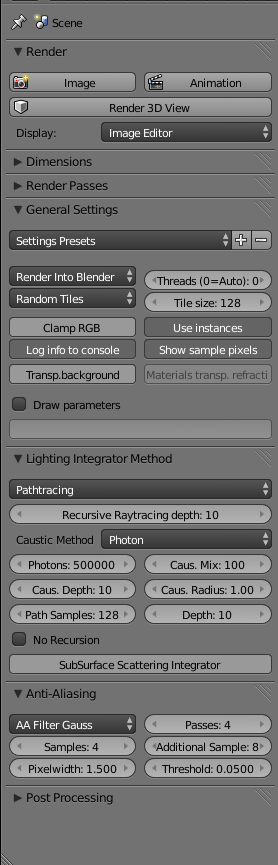
\includegraphics[width=.28\textwidth]{images/generalscreen.png}
    \caption{View of the TheBounty render settings window in Blender, May 2015.}
\end{wrapfigure}

\bigskip

Ray tracing is a rendering technique for generating an image by tracing the path of light through the 3D scene. This technique reproduces the natural behaviour of light and its particular effects on surfaces, such as reflection and refraction, caustics and indirect lighting between diffuse surfaces.

TheBounty usually works as add-on or plugin to a 3D software to provide raytracing capabilities on demand, although it can work as a stand-alone program as well. Blender 3D is the main host application of TheBounty at the moment but there are always on-going projects to add TheBounty support on other 3D packages and modellers.

TheBounty integration in Blender is fairly complete and stable but it should be always considered as a work in progress as Blender and TheBounty keep on evolving. 
}

\section*{TheBounty Renderer features overview}
 \addcontentsline{toc}{section}{TheBounty Renderer features overview}

\paragraph{Lights}
TheBounty supports several types of light sources, i.e. \textit{point}, \textit{spot}, \textit{area} (a rectangular or parallelogram), \textit{mesh} light (which uses a triangle mesh), \textit{sphere} light, \textit{directional} light, \textit{sun} light and \textit{environment}/background light (with importance sampling for efficient image-based lighting, even without global illumination). For more information about the light types, please refer to \tbrref{sec:lights}.

\paragraph{Materials} TheBounty supports \textit{multiple materials} for a single mesh. Materials can consist of different types of materials (diffuse with specular reflection, transparency and translucency)

\todo{Rework this paragraph. This list is really aweful}


\begin{itemize}
\item Multiple materials for a mesh.
\item basic diffuse w. specular reflection, transparency and translucency, support for shader nodes on various properties
\item diffuse+glossy material (Ashikhmin and Shirley), Blinn or anisotropic microfacet distribution w. fresnel effect
\item shader nodes support on diffuse+glossy color, glossiness and bump
\item coated version of the above mentioned, adding specular reflection with fresnel effect (dielectric)
\item basic glass (dielectric) material, with fresnel, filter, absorption and dispersion.
\item emit material
\item export of blender's texture layers as shader nodes
\item blend material, using a blend value or a texture map.
\item subsurface scattering
\end{itemize}

For more information about the different Material options, please refer to \tbrchapref{chapter:materials}.

\paragraph{Textures} Several basic image textures can be used (supported formats are tga, jpeg, png, and even exr and hdr). Also some procedural textures are supported (cloud, marble, wood, voronoi, musgrave, distorted     noise and ``RGB-cube").

For mapping textures to meshes, TheBounty supports multiple textures for a shader, UV coordinates, flat, cube, tube, sphere in global and relative coordinates, blending modes and stencil.  

For more information on this topic, please refer to \tbrchapref{chapter:textureinput}

\paragraph{Backgrounds} TheBounty supports multiple types of backgrounds: single color, two versions of a sunsky (from which the second version has a Night mode), texture and image based lighting and a simple gradient. For more information on this topic, please refer to \tbrref{chapter:backgroundsettings}

\paragraph{Cameras} Different types and settings for camera's can be chosen; a \textit{perspective} camera with raytraced DOF, an \textit{architect} camera with raytraced DOF, an \textit{orthographic} camera and an \textit{angular} camera. For a description and usage of the different camera types, cfr. \tbrref{sec:camerasettings}

\paragraph{Lighting methods} TheBounty gives access to different raytracing lighting methods; direct lighting with support for ambient occlusion and caustic photon maps, path tracing, photon mapping with final gather, bi-directional path tracing and stochastic progressive photon mapping (SPPM).

\paragraph{Volumetrics} TheBounty is able to raytrace volumes, like smoke or clouds. For more information refer to \tbrchapref{chapter:volumetrics}

\paragraph{Adaptive antialiasing} TheBounty supports adaptive (simple color threshold based) antialiasing using variable size reconstruction filters (box, gauss and mitchell-netravali).

\paragraph{Other features} TheBounty also has support for Transparent shadows, multithreaded rendering passes, multipass rendering, radiance map creation. It also has an exporter for XML files (using libXML) for scenes (see YafaRayXML for specifications) and TheBounty is completely plugin based.

\section*{Project History}
 \addcontentsline{toc}{section}{Project History}
The \textit{YafRay} (``Yet Another Free Raytracer'') project was created in 2001 by Alejandro Conty Estévez, and the first public release was in July 2002. These are Jandro's recollections from those years:

\begin{quotation}
\textbf{YafRay}

Introduction

Relevant to Blender v2.31

by Alejandro Conty Estevez,

By the time I started working with YafRay, I was checking out some blender exporters like BMRT and Lightflow. While I was writing some exporting and shading code, I began to be interested in how a raytracer could be written. So when the exams season was in full swing, I became bored (as weird as it may sound) and began to write the main program structure. Once I got a few test renders, I put it off for a year, till the next summer. Then, I wrote the XML loader and YafRay, called "noname" by that moment, began to be an usable program.

Alfredo joined the development almost at the same time. That was of great help. A month later a lot of necessary stuff, like acceleration, were finished and Alfredo ported a lot of his code to YafRay. As the famous hemilight.

Then Luis Fernando Ruiz, a friend of mine and classmate joined to give us a good web site. So we said good bye to that boring plain text web site. We also had the chance to see YafRay rendering on several computers concurrently when Luciano Campal wrote his hack to make YafRay able to work in a distributed way thanks to mosix. It was very exciting when we got access to a 20 computers room for testing. Things started to look very promising when Andrea came with Yable. An experimental export script for an experimental renderer that resulted in a very long thread of cool images at elYsiun. We saw the first nice images done with Blender and rendered with YafRay thanks to him.

We didn't expect that boom. Neither Alfredo nor me. Of course it was the cool export script what was catching people, exporting easily from Blender to a raytracer. We got very excited with all that support from the community. I still get impressed by what people can do with a simple tool like this.

Now more people are getting involved and helping. We begin to have a good documentation section and resources, most of which have been written by Chris Williamson. Basically, it's what you'll see in this chapter. But he is not the only one. YafRay is also getting very easy to use from Blender thanks to Johnny Matthews. I think he spends almost every minute writing Extractor: a new export script for blender. It makes the exporting much more easy by getting all the data directly from blender with nearly no user interaction.

The current power of Extractor and its fast development point out that this could be the future official export scheme for exporting from blender. Anyway, efforts are being made to write a built-in exporter in blender. Alfredo contributed with a lot of shading compatibility code and did some experiments. So it seems we will be able to compare both python and built-in solutions at some point.

YafRay started as an experiment and still is. It's not finished and lacks a lot of features if you compare it with other render engines. I always think is not good enough and that it is hard to imagine what do people see in it. Since people like it for some reason, we now want to really convert it into a full rendering engine that deserves to be called "renderer". This will take some time to have fun coding. We want to add what YafRay lacks (particles, effects, etc...) and to improve global illumination. But only Alfredo De Greef and me are coding YafRay right now, so in order to keep the development up to an acceptable rate, we should get more people to code, more developers. I hope this happens sooner or later.

Finally, I want to thank all the Blender community that supported this project. All those beautiful pictures are what really bring people to YafRay. Likewise, thanks to all the people who give ideas and thoughts on the forums to improve YafRay, and to Juan David G. Cobas for his very appreciated math support.
\begin{flushright}
by \textit{Alejandro Conty Estevez, Chris Williamson, Johnny Matthews}
\end{flushright}
\end{quotation}

By request from the Blender Community, YafRay was added as a Blender plugin from the 2.34 release on, in August 2004. Alejandro de Greef (eeshlo) coded most of the features in the late YafRay releases. At that time it was already evident that a code refactor was necessary in order to add new advanced features to YafRay. The last YafRay release was the 0.0.9 version in Summer 2006.

\begin{wrapfigure}{l}{0pt}
    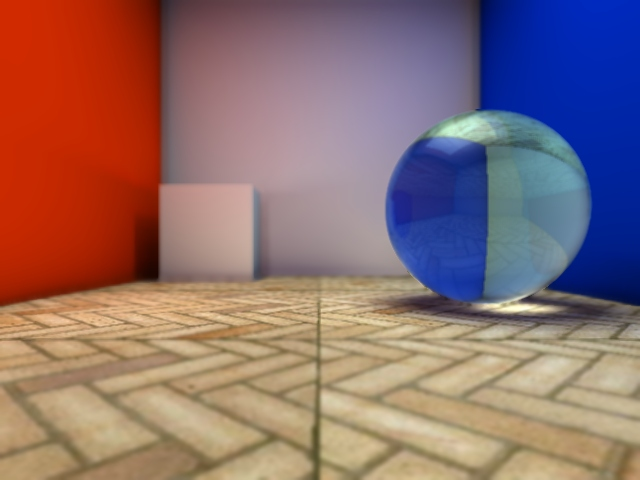
\includegraphics[width=.5\textwidth]{images/caurad_test.jpg}
    \caption{One of the first YafRay renders by \textbf{Jandro}, circa 2001}
\end{wrapfigure}

\textit{YafaRay} is the result of rewriting the YafRay source code from scratch. Mathias Wein (Lynx) started to work on the new engine in December 2005. As a result of the rewriting and to make people aware that it was actually a completely new engine, the YafRay name was changed into YafaRay. Nobody knows for sure what the added 'a' stands for.

\begin{wrapfigure}{r}{0pt}
    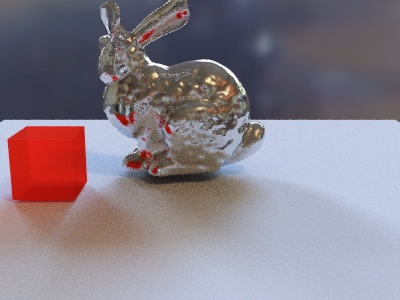
\includegraphics[width=.5\textwidth]{images/bunny_ibl.jpg}
    \caption{One of the first YafaRay renders by \textbf{Lyxn3D}, circa 2005}
\end{wrapfigure}

\bigskip

\textit{TheBounty Renderer} was started by povmaniaco and supported by others when the YafaRay project seemed to start lacking development in 2014. The main objectives of this project are continuing the support for newer Blender versions, optimization and finishing and improving the subsurface scattering.

\input{renderoutput}
\chapter{Objects, Lights and Camera settings}\label{chapter:olc}
In general, settings under these three section of the YafaRay UI are used to give specific YafaRay properties to meshes, light sources and cameras in the Blender 3D scene. The general workflow is:
\begin{enumerate}
\item Create or select an existing object (mesh, light or camera) in the 3D scene.
\item Give it YafaRay specific settings using the YafaRay UI.
\end{enumerate}

\section{Object (meshlight)}
With this feature, a whole mesh in the 3D scene can act as an area light source. The soft shadows produced by area lights need to be sampled several times and then interpolated to reduce noise. This type of light takes more time to render in contrast with point light types such as spot and point.

First of all, you must select the mesh you want it to act as a light source. Then you must enable Object data panel. Finally you must activate the Enable Meshlight button in the YafaRay Object Properties secion. To change the light color, just click on the rectangle next to Meshlight color to open a Color Picker.

\begin{description}
\item[Meshlight color rectangle] opens a Color Picker.
\item[Power] intensity multiplier for meshlight color.
\item[Double Sided] considers both sides of every face as area light.
\item[Samples] defines the amount of samples taken to calculate the soft shadows. The more samples, the less noisy the shadows but the longer it will take to render. The total amount of light sampling depends as well on the anti-aliasing settings, as explained in this section.
\end{description}

\missingfigure{Example of Meshlights, rendered with Bidirectional.}

\todo{Related articles, see yafaray documentation}

\section{Lights} \label{sec:lights}

Lights settings are now fully controlled by the YafaRay UI. The general workflow is creating or selecting a light in the 3D viewport and then editing its properties using the Lamp data section. Users can edit lamp type, color, power, shadows sampling, geometry, etc. It is worth rememberting that lighting power is in fact a product of a couple of settings, Color and Power, available for every light type.

\subsection{Point and Sphere}

In YafaRay there are two options to reproduce omnidirectional lighting which are Point and Sphere. A Point light is a typical omni directional point light source as in Blender Internal with hard shadows, while a Sphere light is a spherical area light source which can produce soft shadows.

The Sphere light settings are:
\begin{description}
\item[Light color rectangle] opens a Color Picker.
\item[Power] intensity multiplier for light color.
\item[Radius] sets the radius of the Sphere light in Blender units.
\item[Create and show geometry] area light gets rendered visibly.
\item[Samples] defines the amount of samples taken to calculate the soft shadows. The more samples, the less noisy the shadows but the longer it will take to render. The total amount of light sampling depends as well on the anti-aliasing settings, as explained in this section.
\end{description}

\missingfigure{Comparison between point light (left) and spherelight (right). Notice the different shadows.}

\subsection{Directional and Sun}

In YafaRay there are two options to reproduce sun lighting which are Directional and Sun.

\smallskip

\paragraph{Directional} light is a traditional sun light model which produces parallel rays and hard-edged shadows.
\begin{description}
\item[Light color rectangle] opens a Color Picker.
\item[Power] intensity multiplier for light color.
\item[Infinite] if enabled, area covered by the directional light is infinite. If disabled, light fills a semi-infinite cylinder.
\item[Radius] if infinite is disabled, radius of the semi-infinite cylinder for directional light.
\end{description}

\paragraph{Sun} light is a more advanced concept and will help us to get blurred-edged shadows when the shadow itself gets away from the casting object, as in real life. The Angle button sets the visible area of the sun. Real sun is visible in a cone angle of about 0,5º. A bigger angle mean a bigger sun, as well as softer shadows, which could be interesting for dawn or sunset scenes. A very big angle can be used to simulate sun light filtered by an overcast sky.
\begin{description}
\item[Light color rectangle] opens a Color Picker.
\item[Power] intensity multiplier for light color.
\item[Angle] visible size of the sun light. Affects shadows.
\item[Samples] it defines the amount of samples taken to calculate the soft shadows. The more samples, the less noisy the shadows but the longer it will take to render. The total amount of light sampling depends as well on the anti-aliasing settings, as explained in this section.
\end{description}


\missingfigure{Comparison between Directional (left) and Sun (right). Notice how, with a Sun light, shadows get blurred as the distance with the casting object increases.}

\subsection{Area}

Arealight is a area light type that can produce soft shadows and its shape can be seen in reflective surfaces. The arealight shadows need to be sampled several times and interpolated to reduce noise in shadows. This type of light takes more time to be computed in contrast with point light types such as spot and point.

Area light size can be controlled in the Area Shape section although you can scale lamp size in the 3D viewport as well. When Create and show geometry is enabled, a rectangle in the size of the area light is generated, so that the area light gets rendered in camera and on reflective components. More lighting power is added as well to the scene. When pathtracing is used, the Create and show geometry option also creates caustics paths, although there exist an option to not trace caustics paths with path tracing as they tend to be extremely noisy (`none' option in Pathtracing settings, see 5.1.1).

\begin{description}
\item[Light color rectangle] opens a Color Picker.
\item[Power] intensity multiplier for arealight color.
\item[Create and show geometry] area light gets rendered visibly. In path tracing, it shoots caustic path rays.
\item[Samples] defines the amount of samples taken to calculate the soft shadows. The more samples, the less noisy the shadows but the longer it will take to render. The total amount of light sampling depends as well on the anti-aliasing settings, as explained in this section.
\end{description}

\missingfigure{Example of a rectangular visible arealight.}

Related articles:

First anti-aliasing pass.
Glossy reflection sampling.

Other area light types:

Spherelight.
Meshlight.

\subsection{Spot}

Spot is a common omnilight within a directional light beam. It has got a feature to blur shadows which could be useful when this light type is used as a sun light substitute in some photonmapping scenes.

\begin{description}
\item[Light color rectangle] opens a Color Picker.
\item[Power] intensity multiplier for spotlight color.
\item[Soft shadows] enables soft-edged shadows.
\item[Samples] defines the amount of samples taken to calculate the soft shadows. The more samples, the less noisy the shadows but the longer it will take to render.
\item[Shadow fuzzyness] fuzzyness of the soft shadows (0 - hard shadows, 1 - fuzzy shadows)
\item[Photon only] it shots photons for indirect lighting and caustics in photon mapping methods but it is not sampled for shadows calculations.
\item[Size] angle of the spotlight beam.
\item[Blend] beam edge gradient.
\item[Show distance and clipping] draws in the 3D viewport spot distance and clipping (Blender Internal features).
\item[Distance] controls fall-off distance (Blender Internal feature).
\item[Clip Start] controls shadow map starting point (Blender Internal feature).
\item[Clip End] controls shadow map limit (Blender Internal feature).
\item[Show cone] draws spotlight cone in the 3D viewport (Blender Internal feature).
\end{description}

In the bottom section of the spot light panel YafaRay developers have included Blender Internal spotlight geometry settings (Distance, Clip Start, Clip End, Show Cone) for more cues in beam directional control.

\section{Camera settings}\label{sec:camerasettings}

The general workflow is creating or selecting an existing camera in the 3D viewport and then editing its properties using the Camera data section. There are four camera types in YafaRay: Architect, Angular, Orthogonal and Perspective.

\subsection{Architect/DOF}

This camera type works like a Perspective camera type, the only difference is that the vertical component of the perspective effect is neglected, so scene vertical lines are not convergent. Depth of Field settings are available for this camera type as well. DOF settings are explained in the Perspective/DOF section.

\missingfigure{Comparison between Perspective (left) and Architect camera (right). Notice the lack of vertical convergence in the Architect camera. Scene by Kronos}
\subsection{Angular}

A camera type useful to produce up to 180 degree panoramas, like the ones produced by fish eye cameras. Alternatively this camera type can be used to create a nice perspective distortion in your renders. Results with this camera type are controlled by two factors: distance to the subject and angle of view.


\missingfigure{Angle of view of a camera}

\begin{description}
\item[Angle] Horizontal opening angle of the camera, takes into account camera aspect ratio to calculate the vertical opening.
\item[Max Angle] Diagonal opening of the circular render.
\item[Mirrored] Mirrors the render in the x direction, as the reflections on a light probe.
\item[Circular] Creates a circular render and shades areas outside.
\end{description}

\missingfigure{Example of an angular camera, used to create perspective distortion. Scene by Gabich.}

\subsection{Orthogonal}

A camera type that renders an orthographic (perpendicular) projection of the scene, without perspective effects. Camera only setting is:
\begin{description}
\item[Scale] Specify the scale of the ortho camera, to control camera zoom.
\end{description}


Comparison between perspective camera (left) and ortho camera (right).
\subsection{Perspective/DOF}

Perspective is the standard camera mode that simulates a lenses photographic camera with perspective effects. All settings available for this camera type are used to enable and configure the depth of field (DOF) effect. The depth of field is the distance that objects appear in focus. DOF settings are:

\begin{description}
\item[Focal Length] distance from the focal point to the image plane in milimeters, to control camera zoom and perspective.
\item[Aperture] The size of the aperture determines how blurred the out-of-focus objects will be. A rule of thumb is to keep it between 0.100 and 0.500 (0 disables DOF).
\item[Obj] Enter the name of the Blender object where the scene will be in focus.
\item[Distance] set the point in which objects will be in focus.
\item[Bokeh type] controls the shape of out of focus points when rendering with depth of field enabled (blur disk). This is mostly visible on very out of focus highlights in the image. There are currently seven types to choose from.
\item[Bokeh bias] controls the accentuation of the blur disk. Three types available, uniform, center or edge, with uniform the default.
\item[Bokeh rotation] rotation of the blur disk.
\end{description}

The DOF effect depends also on the render anti aliasing settings to get a nice blurred effect. First of all it is recommended to lower AA threshold a bit, but not set it to totally zero. Setting a high number of AA passes is also not really going to make all that much difference, the main smoothness factor that makes the most difference is really the amount of AA samples. A single pass with a high number of samples may be sufficient.

\paragraph{Camera Shift}
Technically speaking, this feature shifts the image plane with respect to the focal point so the former is not longer centered. Useful for camera matching work.

\paragraph{Camera Clipping}
Sets the camera clipping limits. Only objects within the limits are rendered. If Limits in the Display panel is enabled, the clip bounds will be visible as two yellow connected dots on the camera line of sight. Useful to make focal lengths compatible with scenes, as explained here,

\chapter{Textures and Texture Mapping}\label{chapter:textureinput}

One of the main points of the old YafRay was the close support of Blender Internal texturing features, and YafaRay keeps this tradition. In general, YafaRay supports:
\begin{itemize}
\item Multiple texture channels for modulating a material component.
\item Procedural textures for color and scalar texturing.
\item Image files (even HDR input) for color and scalar texturing.
\item Several texturing coordinates models and mapping parameters.
\end{itemize}

Like in other 3D rendering packages, there are two main types of texturing: color and scalar. Color texturing is used to modulate color in a material component that allows such an input: diffuse color, mirror color and glossy color. Scalar texturing is performed in material components that do not require color information but a quantity: bump, mirror amount, transparency amount, translucency amount, glossy amount and blending amount. In scalar texturing RGB values are automatically transformed into scalar values (greyscale) ranging from 1 (white) to 0 (black). It is better to use textures in grayscale mode to do scalar texturing in order to make results more predictable.
\section{Texture Channels}

YafaRay supports multiple texture channels for each material component and for relief mapping. Blender principles are observed here: each channel can have its own individual mapping settings and the lower channel in the stack has got priority over the upper one. For instance, a decal should be in a lower channel than a color texture affecting the whole mesh. Also textures blending operations work from bottom to top.
\section{Procedural Texture Type.}

A procedural texture is a computer generated image produced by an algorithm, intended to create a realistic representation of natural elements such as wood, marble, granite, metal, stone, and others.

Procedurals can be used as a color texture or as a scalar texture in any of the mapping options available. Colors in a procedural texture are defined by two controls: Color Picker in the YafaRay Influence (Map to) panel and material diffuse color in the Material section.

Procedural textures supported are: Distorted Noise, Musgrave, Voronoi, Marbre, Wood, Clouds, and Blend. Besides, there is an additional "RGB-cube" procedural type only available by XML output.
\subsection{Noise Basis}

Noise Basis, which is a setting available for most procedural types, governs the structural appearance of the procedural texture. Noise Basis types available in YafaRay are:

These are the settings supported in each procedural type:
\todo{These constructions are weird, have to look at them and insert images}
\subsection{Clouds}

Useful for soft bump mapping of irregular surfaces.
\begin{description}
\item[Soft/Hard noise] Noise strength.
\item[Noise Size] sets scaling for noise.
\item[NoiseDepth] Depth of calculation, the higher the more detail for noise.
\item[Noise Basis] basis used for turbulence.
\end{description}

\subsection{Marble}

Useful for marble. ;)

\begin{description}
\item[Sharpness (soft, sharp, sharper)] Noise definition.
\item[Shape (sin, saw, tri)] band type.
\item[Soft/Hard noise] Noise strength.
\item[Basis] basis used for turbulence.
\item[Size] sets scaling for noise.
\item[Depth] Depth of calculation, the higher the more detail for noise.
\item[Turbulence] amount of turbulence for bands.
\end{description}

\subsection{Wood}

Useful for basic bands and noise with a structure.

\begin{description}
\item[Bands/BandNoise] the procedural is arranged in bands.
\item[Rings / RingNoise] the procedural is arranged in rings.
\item[Shape (sin, saw, tri)] band type.
\item[Soft / Hard Noise] Noise strength.
\item[Size] sets scaling for noise.
\item[Turbulence] amount of turbulence for bands or rings.
\item[Noise Basis] basis used for turbulence.
\end{description}

\subsection{Musgrave}

Very flexible. Useful for terrain and rock surfaces. The \textbf{Intensity Scale} control is useful to localise the result.

\begin{description}
\item[Musgrave type] fractal noise algorithm (Hetero Terrain not supported).
\item[Dimension] contrast between consecutive layers, for detail.
\item[Lacunarity] gap between layers.
\item[Octaves] layers of noise used.
\item[Intensity] overall intensity of texture.
\item[Noise Basis] basis used for turbulence.
\item[Size] sets scaling for noise.
\end{description}

\subsection{Voronoi}

Voronoi is a procedural type with a cellular look. Very flexible. Useful for organic surfaces.

\begin{description}
\item[Distance Metric] shape of the cells.
\item[Coloring] color of the cells.
\item[Intensity] overall intensity of texture.
\item[Size] cell size.
\item[Feature Weights (1, 2, 3, 4)] defines distances between each cell.
\end{description}

\subsection{Distorted Noise}

Complex and versatile.

\begin{description}
\item[Distortion] amount of distortion.
\item[Size] sets scaling for noise.
\item[Noise Distortion] basis used for distortion.
\item[Noise Basis] noise to distort.
\end{description}

\subsection{Blend}

Gradient effects and for stencil.


Related articles:

Material Modulation.
Volume types.
The NoiseVolume Texture

\section{Image Texture Type}

Texture input is done by selecting Image as a Texture Type and loading the image in the `Map Image' panel. You can use several texture channels for modulating just one component or several ones. YafaRay 8-bits supported formats are tga, jpeg and png. YafaRay also supports 16-bits tiff, exr and hdr.

\begin{description}
\item[Source] Single image and Image Sequence are supported.
\item[Input Color Space] Use sRBG for 8-bits formats and Raw for high dynamic range formats.
\item[UseAlpha] Renders the texture alpha channel as transparent (if it exists), white otherwise. Enabled by default.
\end{description}

\note{YafaRay can not load Blender encapsulated textures. If your Blender file has got encapsulated data, you must unpack first (File\textrightarrow{}External~Data\textrightarrow{}Unpack). YafaRay will load textures from the created `textures' folder.

During the rendering process, the Blender back console shows up messages when a texture image can't be loaded by YafaRay. Pay attention to them!

If your file is unpacked but YafaRay can't load textures, be sure that the path selected in the 'Image' panel points to the actual location of the file in your HD.}
\subsection{Image Sampling and Image Mapping}
\begin{description}
\item[Flip X/Y Axis] flips the texture's X and Y axis.
\item[UseAlpha] Renders the texture alpha channel as transparent (if it exists), white otherwise.
\item[CalcAlpha] transform RGB values into amount of transparency, for mapping transparency or translucency in the shinydiffuse material.
\end{description}

Texture extension:

\begin{description}
\item[Extend] the colour of the edge is extended outside the image.
\item[Clip] an alpha value of 0.0 is returned outside the image. This allows you to 'paste' a small logo on a large object.
\item[Clipcube] outside a cube-shaped area around the image, an alpha value of 0.0 is returned.
\item[Repeat] The image is repeated horizontally and vertically as often as set in Xrepeat and Yrepeat
\item[Checker] a checkerboard is made. Mortar governs the distance between the checkers.
\item[Xrepeat, Yrepeat] sets a repetition multiplier in the corresponding direction.
\item[Crop Mix X, Y - Crop Max X, Y] Use these to crop, or choose a portion of the texture.
\end{description}

\section{Object Mapping Coordinates}

Coordinates supported:
\begin{description}
\item[Global] the texture uses the scene's Global 3D coordinates for mapping.
\item[Object] Uses a child Object's texture space as source of coordinates. The Object name must be specified in the text button on the right. Often used with Empty objects.
\item[UV] UV coordinates are used for texturing.
\item[Generated] the texture uses the object's local space.
\item[Win] the texture uses the screen coordinates.
\end{description}

Projection modes:

\begin{description}
\item[Flat, Cube, Tube, Sphere] use them depending on the overall shape of the object. Use Flat for UV mapping.
\end{description}

Other settings:

\begin{description}
\item[Offset X, Y, Z] moves the texture.
\item[Size X, Y, Z] scales the texture.
\item[X, Y, Z axis] Re-orders the X, Y and Z coordinates.
\end{description}

\missingfigure{The image above is an example of Generated coordinates mapping and object projection. Notice how the texture adapts to the objects position and size. Besides, each object is using a suitable projection mode, so each surface is perpendicularly mapped.}

\section{YafaRay Influence (Map To)}

\begin{description}
\item[Modulation modes (Diffuse color, Mirror amount, Mirror color, etc.)] the texture modulates the material property selected. Modes supported depend on the YafaRay material used (see it in the materials modulation section). Negative mode is supported. More than one modulation mode can be selected; in this case different material properties will be modulated with the same texture channel. Displacement mapping is only supported through a mesh modifier (more info here).
\item[Blending modes] How this channel interacts with other channels above it. Supported modes are mix, add, multiply, substract, screen, difference, darken, lighten. More info here.
\item[Stencil] the texture is used as a mask for all following textures. More info in \tbrref{sec:stencil}
\item[Negative] produces a negative of the texture.
\item[No RBG] Converts a texture into a gradient, the two extremes of the gradient scale being Material main color and color set in Color Swatch.
\item[Color Swatch] A sort of a secondary color, to be mixed with Material diffuse color in procedural textures and in the No RBG feature.
\item[Dvar] default value for scalar type textures (Mirror Amount, Transparency, etc..)
\end{description}
\todo{All the ``more info here'' should get a \textbackslash{}tbrref}

\subsection{Stencil} \label{sec:stencil}

Stencil is a texturing feature that allows for mixing two texture channels in a controlled way, by using an intermediate mask texture. This feature can be used as well to set invisible parts of a texture, by using a stencil channel below. White value in the mask texture renders the above texture channel invisible.

The images above show an example of a stencil setup. On the left there are the textures used and on the right the texture channels arrangement.

The image above shows the `Map to' panel of the stencil texture channel. Notice that the Diffuse Color, Stencil and No RGB buttons are enabled.

\missingfigure{The final result.}
Related articles: Material Modulation.

\subsection{Blending modes}

Blending modes are used to determine how two texture channels are blended into each other. The default blend mode is Mix, which is used to hide the upper channel with whatever is present in the lower channel (remember that in Blender, textures have a higher visibility priority the lower they are in the channels stack). However, as each pixel in a texture has a numerical representation, a large number of mathematical ways to blend two channels is possible.

This feature can be used to add complexity and richness to your texturing works. Supported modes are mix, add, multiply, substract, screen, difference, divide, darken and lighten.


We are going to blend two textures: on the left is the base texture, on the right the blend texture. Please look at them carefully.


\missingfigure{Base texture}   \missingfigure{Blend texture.}

Add

A very basic blending mode. It simply adds pixel values of one channel with the other (a+b). In case of values above 1, white is displayed. This mode is commutative (base and blend channels can be swapped)

Notice how the black values in the blend texture don't affect the base texture, since a+0=a

Subtract

This blend mode simply subtracts pixel values of the base channel with the blend channel (a-b). In case of negative values, black is displayed.

Notice how black values in the blend texture don't affect the base texture since a-0=a, while white values produce a black result.

Multiply

Multiply is a basic blending mode for darkening areas of a texture.

Pixels from both channels are simply multiplied by each other. This returns a darker result than both input parameters, except if one of them equals to 1 (white). Completely white values do not change the base texture at all (and vice versa) - completely black values give a black result.

This mode is commutative (base and blend channels can be swapped)

Screen

Screen is a basic blend mode for lightening areas of a texture.

It is the opposite of 'multiply' mode. It returns a brighter result than both input parameters in most cases, except if one of them equals 0 (black). Completely black values in the blend channel do not change the base at all (and vice versa) - completely white gives a white result.

This mode is commutative, channels can be swapped.

Difference

Subtracts either the blend texture from the base texture or the base texture from the blend texture, depending on which is brighter, to get always a positive result. Blending with black produces no change as a-0=a. Blending with white inverts the picture (1-a).

This kind of blending produces a lot of variation. This mode is commutative as well.

Divide

This mode simply divides pixel values of the base texture with the blend texture (a/b). The darker the blend texture is, the lighter the result. However, remember that it is not a linear function, so the result easily reaches the upper limit with regular factors, since $\tfrac{a}{0}=\inf$.

Darken

Pixels from both channels are compared to each other, the darkest one is taken.

Lighten

Pixels from both channels are compared to each other, the lightest one is taken.

\chapter{Materials} \label{chapter:materials}
In order to understand Yafaray materials it is always better to think of it as a sum of components rather that a global calculation. Once the eye rays are shot, a render engine is always tracing different kind of rays according to surface properties defined in the materials section. These rays fall into 5 main categories: diffuse, mirror specular, glossy specular, mirror refraction and glossy refraction. A YafaRay material is usually a combination of several of these basic components.

\section{Multimaterial}

YafaRay supports Blender Multimaterial feature, which means that you can assign different materials to different parts of a mesh, using sets of polygons. You can find more information about multimaterials here on \url{http://wiki.blender.org/index.php/Doc:2.6/Manual/Materials/Multiple\_Materials}.

Alternatively you can use the Blend material to mix two materials in a mesh. In YafaRay, there are three ways to mix material properties in an object, which are:

\begin{description}
\item[Stencil] to mix two texture channels in a material, using a texture as a blending pattern. (for more information, refer to \tbrref{sec:stencil})
\item[Blend material] to mix two materials in a mesh, using either a blend factor or a texture.
\item[Multimaterial] to assing different materials to a mesh, using sets of polygons.
\end{description}

\section{Material settings}

There are five generic material types in YafaRay, with many possibilities for each of them to achieve advanced effects. They are glass, rough glass, coated glossy, glossy and shinydiffusemat. Also, there is a Blend type to mix two of them in a controlled way. This is a brief list of what YafaRay materials can be useful for:

\begin{description}
\item[Blend] blend two materials, using a blend factor or a texture map.
\item[Glass] glass, water, fake glass.
\item[Rough Glass] rough transparent materials.
\item[Glossy] all kind of plastics, clean and polished metal, clean rough metal, car paint, finished wood, lacquered surfaces, painted surfaces, varnished wood, glaze and organic surfaces, materials with anisotropic reflections.
\item[Coated glossy] car paint, lacquered surfaces.
\item[Shinydiffusemat] stone, rusted metal, concrete, fabric, paper, rough wood, curtains, emit surfaces, perfect mirror, materials with a basic transparency and alpha mapping with color-filtered shadows, translucent materials with color-filtered shadows, etc.
\end{description}

To aquire some background knowledge about the topics explained in the following sections, take a look at Neil Blevins's webpage \footnote{\url{http://www.neilblevins.com/cg_education/cg_education.htm}}.

\section{Material Preview}

With this feature you can render a little preview of the material selected. The material preview will be rendered with the YafaRay engine and according with the material parameters choosen, and will take into account material mapped textures.

\section{Glass}

To render correct glass, it is important that glass objects follow realistic techniques for modelling, such as closed meshes with real thickness.

It is also important that your mesh normals point in the correct direction. Use the normal tools in Blender to control normal direction.

In real life, light refracts one time when passing from one medium to another, for instance from solid (glass) to liquid. In your 3D scene, use one mesh for each refractive event. That means: water meeting glass must be exactly one surface, and the relative refration index of the "water meets glass" surface must be $\frac{\text{IOR}_{glass}}{\text{IOR}_{water}}$ (when normals are pointing into the water). Taking into account that glass IOR is 1.55 and water IOR is 1.33, a cross section of a glass of water should look like the glass cross section on the left (normals in red).

Rendering a a number of consecutive transparent surfaces depends on recursive raydepth (General settings, Render main section). If a transparent surface is rendered black, try increasing Raydepth.

Glass is basically refraction, reflection and absorption of incoming light. It means that the scene sorrounding the glass has got an impact on the glass appearance, as well as the lighting setup. It means that glass will produce caustics if certain conditions are met, which are:

\begin{itemize}
\item There exist a light source and/or a background (IBL, Sunsky) which is shooting caustic rays.
\item The glass material has got $\text{IOR}>1$.
\item A global illumination method is used (pathtracing with caustic paths, photonmapping, bidirectional) or Use caustics is enabled in the Direct Lighting method.
\item The caustic rays have enough depth to pass through all the transparent surfaces (Caustics depth).
\end{itemize}

Glass material mixes several independent concepts that can be used alone or combined with the other parameters to get diferent kinds of results. These concepts are:

\paragraph{Absorption}

Some of the incident light is absorbed by a transparent medium. The more distance light has to get through a medium, the more it gets absorbed. In a glass with different sections, the glass will get darker if the section is bigger.

Absorption also defines the color of the glass and the strength of the caustic effect. The more light is absorbed, the less light is transmitted. By using an absorption color, we also define the color of caustics. White disables absorption.

\paragraph{Filtering}

Color is uniform regardless of glass section. The amount of transmitted light is also constant. You can use this setting instead of absorption if the glass section is uniform, for instance.

You need to use this setting to tint transparent shadows when Fake Shadows and Transparent Shadows are enabled.

Transmit Filter is a related setting which blends Absorption and Filtering. When Transmit Filter equals 1, Filtering is shown. When Transmit Filter equals 0, Absorption is shown (if enabled).

\paragraph{Reflection (Mirror)}

Some of the light is reflected. Amount of reflection depends on the index of refraction (IOR). The higher the index, the more reflective the glass is. It produces reflective caustics.

\paragraph{Refraction (IOR)}

Refraction is the change in direction when light waves travel from a medium with a given refractive index to a medium with another. Refraction produces caustics. Some materials index are:

Ice: 1.31
Water: 1.33
Clear plastic: 1.40
Standard glass: 1.52
Amber: 1.55
Diamond: 2.42


\paragraph{Dispersion}

Dispersion causes the spatial separation of a white light into components of different wavelengths (different colors).

When Path tracing is used, dispersion noise depends on path tracing samples, the more the samples the lesser the noise.


\paragraph{Fake Shadows}

Not all light tracing methods are optimised to render caustics. This is the case of Direct lighting or Path tracing for instance. When fake glass is enabled, raytracing shadows rays get through this object when looking for light sources to sample, and colored transparent shadows are calculated based on Filtering values. Notice the glass shadow, compared with the examples above.

The Transparent Shadows button in the Render section must be enabled too for this feature to work. Filter color controls color of the transparent shadows.

Related articles:

Ray Depth.
Shadow Depth and Transparent shadows.
Caustic Photon Map.
Rendering Pathtracing caustic component.
Photon Mapping.

\section{Rough Glass}

This is basically a glass material (see section above) but using a glossy model for the refractive component. As with the glossy material, tiny random bumps on the surface of the material cause both the reflective and the refractive components to be blurry. Exponent controls blur of the glossy refraction; the higher the exponent, the rougher the surface is. The glossy effect can be reinforced by using a fine relief map. Sampling of the glossy effect depends on antialiasing settings and it works well with adaptative sampling strategies.


Difference Between Exponent=0.20 (left) and Exponent=0.90 (right). Caustics produced by SPPM.

\section{Glossy}

A glossy reflection means that tiny random bumps on the surface of the material cause the reflection to be blurry. In fact there is a wide range of materials with such a reflection. YafaRay glossy material can be useful for all kinds of finished surfaces such as plastics, polished metal, car paint, finished wood, lacquered surfaces, painted surfaces, varnished wood, glaze, organic materials, etc. The glossy effect can be reinforced by using a fine bump map, or by mapping glossy reflection with a fine texture.

The main concepts of the glossy shader are:

\paragraph{Diffuse and Glossy colors}

A Glossy material has got two colors, diffuse and glossy. Glossy reflection parameter, apart from controlling the reflection strength, should be understood as a blend factor between the diffuse and the glossy color. The more reflective, the less diffuse.

\begin{quote}
"When light hits an object, the energy is reflected as one of two components; the specular component (the shiny highlight) and the diffuse (the color of the object). The relationship of these two components is what defines what kind of material the object is. These two kinds of energy make up the 100\% of light reflected off an object. If 95\% of it is diffuse energy, then the remaining 5\% is specular energy. When the specularity increases, the diffuse component drops, and vice versa. A ping pong ball is considered to be a very diffuse object, with very little specularity and lots of diffuse, and a mirror is thought of as having a very high specularity, and almost no diffuse."
\begin{flushright}
as stated in \textit{Siggraph 96 course notes book \#30 Pixel Cinematography: A lighting approach for Computer Graphics}
\end{flushright}
\end{quote}

When Glossy reflection is zero, you will see mostly the diffuse color with a bit of rim glossy color (image on the left). When Glossy reflection value is 1, you will see only the glossy color (image on the right). Notice Glossy reflection slider in both images:

Remember that coloured reflections is a particular feature of conductive materials (gold, copper), while non-conductive have got white colored reflections. So Glossy color of non-conductive materials like plastic should be white. Diffuse Reflection value is just a diffuse color multiplying factor.

Related articles:

Diffuse color mapping.
Specular color mapping.

\paragraph{Glossy reflection and Exponent}

Glossy reflection controls the strength of the reflection. The more reflective, the less diffuse.

Exponent controls blur of the glossy reflection; the higher the exponent, the sharper the reflection. Use values between 1 and 200 for plastics and higher values for metallic surfaces. Glossy reflection produces caustics.

Below there is an example of a material with different glossy reflection (GR) and exponent settings (EXP). Diffuse color is dark grey and glossy color is white:

Related article: Specular intensity mapping.
\paragraph{Glossy reflection sampling}

When these light sources are used in the scene, noise in the glossy reflection depends on:

Area light (area light, sphere light, mesh light) samples.
Sun light samples.
HDR backgrounds (IBL, Darktide Sunsky, Sunsky) samples.
AA samples, the higher the less noisy.

Below on the right, area lights are using 2 samples while on the left they are using 64 samples.

Related articles:

Arealight
Sun light.
First anti-aliasing pass.
Background Settings.

\paragraph{As Diffuse}

When As diffuse is enabled in Photon mapping, it means that the photon map will be used to calculate the glossy reflection, instead of raytracing it, which results in faster render times. In practice, this method is recommended only for glossy surfaces with a low Exponent, since the precision of glossy reflections calculated with photon mapping is always lower. Besides, As diffuse option enabled will be likely to produce flickering of the glossy reflection in animations.

Both spheres in the left render have got As diffuse enabled and the render time is 166 seconds. Both spheres in the right render have got As diffuse disabled and the render time is 186 seconds. Notice the reflections!

Related articles:

Exponent.
Photon Mapping.

\paragraph{Anisotropic reflections}

This material is useful to get anisotropic reflections, which means that reflection is not equal in all directions. This kind of reflection happens when a defect in a reflective surface repeats with some regularity. When Anisotropic is enabled, the exponent value is divided into vertical and horizontal components. By using a different value for each component., the reflection will take an anisotropic oval shape. This effect can be reinforced by using a suitable bump map. When Anisotropic is enabled, the Exponent button is disabled. Horizontal and vertical direction of the anisotropic exponent depend on UV mapping coordinates. Below you have a comparison between anisotropic reflections (left) and default isotropic reflections (right).

\section{Coated Glossy}

Coated Glossy is basically a glossy material (see the previous section) with some kind of reflective coating layer on top. IOR is the setting that controls reflectivity of the coating top layer. This reflective layer can produce caustics. It is a good material for car paint. Below an example of different IOR values:

Related article: Glossy material.

\section{ShinyDiffuse}

Shinydiffuse is a shader with many applications. It can be useful to get:

Diffuse materials without any specular component.
Perfect mirror reflection with or without Fresnel effect.
Alpha mapping with shadows calculation derived from the map.
Translucency with color filtering.
Transparency with color filtering.
Emit surfaces.

For instance, this material can be used for rough stone, rusted metal, concrete, fabric, clay, asphalt, paper, rough wood, chrome balls, shiny plastics, basic car paint, curtains, leaves, billboards, etc.

The main concepts of the ShinyDiffuse shader are:



\paragraph{Diffuse reflection}

Diffuse reflection is the reflection of light from an uneven or granular surface such that the incident rays are randomly reflected and scattered in all directions. The amount of diffuse reflection is mainly controlled by the surface Color and Reflection Strength. YafaRay uses two models to render the diffuse component, which are Lambertian and Oren-Nayar.
Lambertian is a basic diffuse model with no view dependence. Brightness is constant from all viewing directions; only interaction between surface and light sources is modelled. It is a method valid only for very smooth matte surfaces, like paper, smooth plastic or polished wood.

Oren-Nayar is a view dependent, physically-based microfacet model for diffuse reflections, which takes into account geometric optics and interaction at microfacet level produced by light sources. Oren-Nayar models the diffuse reflectance for rough surfaces more accurately than the Lambertian model. Sigma controls the roughness of the surface.

Diffuse Reflection value is a diffuse color global multiplying factor.


GPL Photograph of a comparison between a matte clay vase and its renderings with the Lambertian model and the Oren-Nayar model (Source). Some Sigma values, as per the official project page for the Oren-Nayar model, are:

\begin{multicols}{2}
\begin{tabular}{l l}
Felt& 0.414686\\
Rough plastic& 0.278057\\
Leather& 0.179776\\
Velvet& 0.751002\\
Pebbles& 0.443289\\
Plaster\_b& 0.543788\\
Rough paper& 0.311376\\
Roof shingle& 0.819147\\
Rug\_b& 0.613889\\
Sponge& 0.872413\\
Wool& 0.978133\\
\end{tabular}
\begin{tabular}{l l}
Quarry tile& 0.360574\\
Slate\_b& 0.309590\\
Human skin& 0.579386\\
Brick\_b& 0.275990\\
Linen& 0.514593\\
Cotton& 0.482679\\
Stones& 1.107168\\
Concrete\_b& 0.308956\\
Concrete\_c& 0.461930\\
Wood\_b& 0.351271\\
Tree bark& 0.293226\\
\end{tabular}
\end{multicols}

Related article: Diffuse color mapping
\paragraph{Mirror and Fresnel}

Mirror produces pure specular reflection. Mirror strength is a blend factor between the specular and diffuse components, with their respective colors. The more specular, the less diffuse component will be shown. When Fresnel is enabled, the amount of specular reflection depends on how the viewer is oriented relative to the surface. Fresnel means that a surface is more reflective at grazing angles than at perpendicular ones. IOR controls the Fresnel reflection strength, the higher the more reflective at every angle. Mirror and Fresnel reflections can produce caustics. Below are several examples of Mirror and Fresnel, MS stands for Mirror Strength. White is being used for both diffuse and mirror color:

Related articles:

Specular color mapping.
Specular intensity mapping.
Ray Depth.

\paragraph{Transparency}

With this setting you can achieve a basic transparency effect, without refraction but with transparent shadows and color filtering.

Transparent shadows and color filtering means that light is filtered by the transparent surface, and gets coloured and diminished according to the surface properties. Transparency is basically a 'fake' feature intended for basic transparency and alpha mapping purposes, since it is a mappable feature. To get tranparent shadows and color filtering, Transparent Shadows button must be enabled in the Settings main section.

Settings that affect this feature are:

Diffuse color Picker: control diffuse color of the object, which results in color filtering.
Transparency: Amount of transparency.
Transmit Filter: color filtering strength. When it equals 0 there is no color filtering, therefore shadows are not tinted by the tranparent surface.

In Settings main section:

Raydepth: for camera rays, to get through successive transparent events.
Transparent Shadows: this option must be enabled to produce transparent shadows and color filtering. Technically speaking, it allows raytracing shadows rays to get through this mesh when looking for light sources.
Shadows Depth: for raytracing shadow rays, to get through successive transparent surfaces.

With this feature you can emulate the Blender OnlyCast feature, which makes objects not to be rendered but to cast shadows only. Set the object transparency=1 while keeping Transparent Shadows button disabled.

Related articles:

Alpha intensity mapping.
Ray Depth.
Shadow Depth and Transparent shadows.
Glass material.


\paragraph{Translucency}

With this setting you can achieve a basic 2D translucency effect with transparent shadows and color filtering. Translucent materials allow light to pass through them but only diffusely; you can not see through. Light is scattered after passing through the transparent surface.

Transparent shadows and color filtering means that light is filtered by the translucent surface, and it is coloured and diminished according to the surface properties. Translucency slider controls amount of translucency.


Scattered light with transparent shadows and color fitering only works with Global Illumination methods, which are Pathtracing, Bidirectional Pathtracing and Photon mapping.
Example of translucency, notice the curtains. `My Room' by ChojinDSL.
Related article: Alpha intensity mapping.

\paragraph{Emit}

Amount of light a material emits, similar to the mesh light concept. Color of the emitted light is controlled by the Diffuse color. Emit slider controls strength of the emitted light.

Emit objects can be used as diffuse light sources, but you will have to use it with path tracing or bidirectional path tracing lighting methods.
Related article: Diffuse color mapping with emit value


\section{Blend Material}

This feature takes two defined materials and mixes them into a third one. You need to define three materials then, two ones to mix and a third Blend material which is applied to the object to render. This feature can be useful to mix properties from two different materials, for instance glossy reflection blended with transparency. It can be useful as well to map two different parts of a mesh with different materials using a texture as a pattern, without resorting to multimaterial which depends on mesh polygons.

Blend value controls the percentage of each material in the final mix. A value of 0.50 means that each material contributes the same to the final look. These are examples of different blend materials; the sphere on the left has got the Blend material:
0.5 blend between a glossy material and a shinydiffuse with transparency=0.85.
0.50 blend between a glossy material and a shinydiffuse with mirror=0.80.
0.25 blend between two glossy materials. One material uses exponent=15, the other uses exponent = 1500.
0.25 blend between two shinydiffuse materials. One uses mirror=0.20 and transparency=0.85. The other is a completely diffuse material.


\chapter{Background settings}\label{chapter:backgroundsettings}

\chapter{Volumetrics}\label{chapter:volumetrics}

\end{document}
